%08/10 - Álvaro
\chapter{Reconocimiento de patrones en imagen biomédica}
\section{Clasificación de imágenes}
\subsection{¿Qué es la clasificación?}
La clasificación busca asignar una etiqueta entre varias categorías o clases a una imagen o grupos de éstas. Se pueden asignar múltiples etiquetas a una imagen (multiestancia).

El algoritmo pasa primero por una fase de entrenamiento y una fase posterior de test e inferencia. El dataset es un conjunto de imágenes de entrenamiento (suele ser supervisado), que implica que el dataset viene etiquetado. Se extraen las características y se entrena con los datos de ejemplo y las etiquetas. De esta forma se obtiene un clasificador entrenado. 

En el test, se proporciona una imagen no existente en el entrenamiento. Se extraen las mismas características que se extrajeron en el entrenamiento aplicando el clasificador obtenido durante la fase de entrenamiento. Esto permite predecir la clase que hay en esa imagen.

\paragraph{Dataset} 
La base de datos se suele dividir en tres conjuntos para poder realizar validación cruzada. Las imágenes de entrenamiento sirven sólo para entrenar el clasificador. El subset de validación no sirve para entrenar, si no para medir el error y ajustar los parámetros. Las imágenes de validación nunca se deben usar para entrenar. Por último están las imágenes test, que dan una medida del error con datos nuevos que nunca se hayan visto. 

\paragraph{Extracción de características}
Las imágenes se deben modelar para extraer las características. Se pueden modelar los píxeles, histogramas de los niveles de gris, patrones (templates) o descriptores de regiones o puntos de interés entre otros.

\paragraph{Entrenamiento}
Se genera una función que obtiene una predicción al ser aplicada sobre características de la imagen.

\subsection{Evaluación del rendimiento}
La precisión de algoritmos de Machine Learning (ML) debe ser evaluada para seleccionar el mejor en cada tarea. 
Una tarea puede ser, por ejemplo, segmentación de tumores cerebrales en imágenes de resonancia magnética (MRI) e identificar qué píxeles son tumor.

Hay tres elementos clave para evaluar la efectividad de algoritmo (de clasificación) de manera sistemática:
\begin{itemize}
\item \textbf{Ground-truth/dataset}: valor o categoría real de cada dato para la tarea específica.
\item \textbf{Resultado}: predicción del algoritmo. Aunque se entrenen en otro dataset, deben ser evaluados en común. Esto significa que si entrenas un dataset de ayuda a la conducción con datos de Alemania, debe valer también para Suecia.
\item \textbf{Métrica}: función que calcula la similitud entre los valores o categorías del resultado y del ground-truth.
\end{itemize}

Hay diferentes modelos de entrenamiento en función de los distintos niveles de anotación. Un entrenamiento sin supervisión no está asociado a la etiqueta. Una supervisión débil define la clase o categoría, y una supervisión completa define los distintos segmentos. 

El resultado es la predicción del algoritmo. Tanto la predicción como el ground-truth son binarios, por lo que hay dos tipos de errores en clasificación: false negative y false positive. 
\begin{itemize}
\item Métricas focalizadas:

$$\text{precisión} = \frac{TP}{TP + FP} = \frac{correctos}{devueltos}$$

$$\text{sensitivity, recall, hit rate o true positive rate (TPR)} = \frac{TP}{TP + FN} = \frac{positivos}{total anotaciones positivos}$$

\item Métricas globales:

$$\text{Accuracy} = \frac{TP + TN}{TP + TN + FP + FN} = \frac{predicciones correctas}{total predicciones}$$

$$\text{Error rate} = \frac{FP + FN}{TP + TN + FP + FN} = \frac{predicciones incorrectas}{total predicciones}$$

$$\text{F-score} = 2 \cdot \frac{precision \cdot recall}{precision + recall}$$
\end{itemize}

Mediante una \textbf{matriz de confusión} se puede visualizar los aciertos y errores para clasificaciones multiclase.

\subsection{Clasificación basada en \textit{bag of words}}
Se aprenden diferentes características visuales que representen un objeto. El objeto se modela como mezcla de elementos básicos o textones. Dependiendo de su textura se van a agrupar de una forma u otra. La bag of visual words tiende a acumular los patrones más repetidos en un diccionario de textones y caracterizar en un histograma las veces que aparecen los textones en la imagen de entrada. No obstante, no se incluye información de localización espacial ni existe distinción entre frente y fondo de la escena, trata todas las texturas por igual. 

Son modelos para describir imágenes (contiene dos ojos, una nariz, una boca), pero no dónde se encontraba originalmente en la imagen (izquierda, derecha, arriba, centro, ...).

Las etapas del modelo son las siguientes:
\begin{enumerate}
\item Extracción de características de las imágenes
\item Aprendizaje del vocabulario visual
\item Cuantificación de características (palabras visuales) a partir del vocabulario visual; se puede limitar a un cierto número, como las 4 palabras visuales más clave, más frecuentes, más distribuidas, etc.
\item Representar imágenes como histogramas con palabras visuales
\end{enumerate}

\begin{figure}[h]
\centering
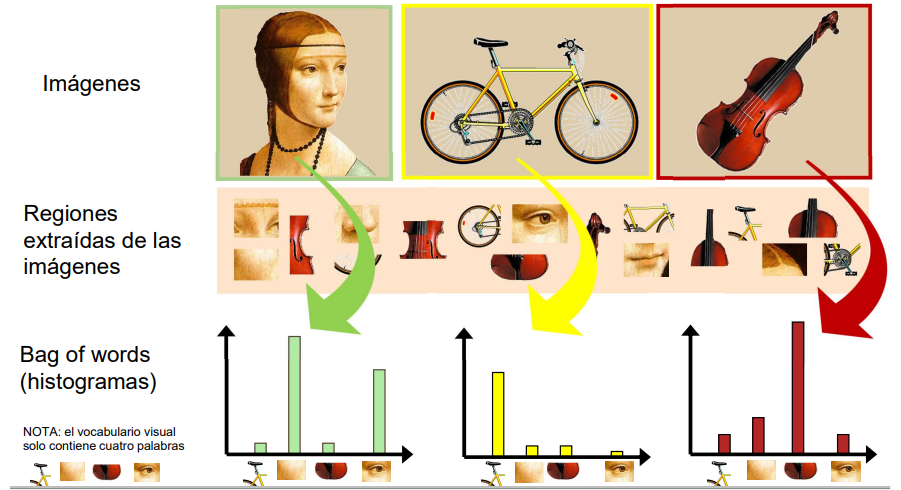
\includegraphics[width = 0.8\textwidth]{figs/bag-of-words.png}
\end{figure}

Este proceso se repite para cada imagen nueva que se encuentre. Todas las imágenes de entrada se matchean con el diccionario visual creado y se busca a la que más se parece. Una vez que se tienen los histogramas, se suele aprender un clasificador para distinguirlas.

\begin{table}[h]
\centering
\begin{tabular}{p{6.5cm}|p{6.5cm}}
Ventajas del modelo Bag-of-words & Desventajas del modelo Bag-of-words \\ \hline
Flexible a la geometría, deformaciones y puntos de vista & El fondo y el primer plano se mezclan al representar toda la imagen \\
Resumen compacto del contenido de la imagen & La formación óptima del vocabulario \\
Proporciona representación vectorial dimensional fija para conjuntos & El modelo básico ignora la geometría; debe verificarse después o codificarse mediante funciones \\
Muy buenos resultados en la práctica & 
\end{tabular}
\end{table}

\section{Detección de objetos}
\subsection{¿Qué es la detección de objetos?}
La detección de objetos permite clasificar y localizar objetos espacialmente en la imagen que discriminen la información del objeto de la información del fondo. La detección de objetos no es la identificación de objetos concretos, si no la clasificación de distintas clases de objeto genéricas.

Presenta muchos desafíos. En el caso de las personas, cada objeto tiene mucha variabilidad: la postura, altura, edad, escala, relación de aspecto, punto de vista más lejano, multitudes, iluminación, ropa. Esto dificulta identificarlos entre ellos.

Entre los criterios de diseño está la búsqueda eficiente de los objetos más probables. Incluso los modelos simples requieren buscar cientos de miles de posiciones y escalas. También se deben diseñar características generalistas y robustas para generar puntuaciones útiles. Para tratar diferentes puntos de vista, a menudo se entrena diferentes modelos para los puntos de vista existentes en la base de datos.

Las etapas generales para la detección de objetos son:
\begin{enumerate}
\item Definir modelo objeto: patrón estadístico. El objeto es un rectángulo en la imagen y se buscan características definidas en el rectángulo (color, textura, forma, iluminación). Se pueden utilizar detección de bordes como Prewitt.

\item Generar hipótesis, proponer un alineamiento del objeto a la imagen: la más utilizada es la ventana deslizante. Se selecciona una ventana (cuadradito) en cada ubicación y escala y se realiza un desplazamiento definido por el parámetro paso (stride). Entre una ventana y otra se puede solapar un 99\%. Tradicionalmente, la ventana se mantiene de tamaño y cambia la resolución de la imagen a un tamaño menor. Así, el objeto que se encuentra debería ser más grande que en la imagen original. Esto permite lidiar con multi-escala o ventanas con diferntes tamaños. Cada ventana obtenida se clasifica independientemente para ver si contiene el objeto a detectar.
 
En la nueva imagen, se obtienen las características asociando los nuevos elementos al diccionario visual. Teniendo una cabeza, se sabe que está en la parte superior del objeto. Así se realiza un votado probabilístico para obtener el centro. Se genera un espacio tridimensional de votación, que es un espacio continuo. La profundidad, el eje z, de ese espacio es la escala de la imagen, si se encontró con el tamaño original o en una menor resolución. 

\item Puntuar hipótesis basado en correlación con el modelo. Se realiza una suma de puntuaciones de características en posiciones fijas y se establece un threshold a partir del cual establecer si es un objeto de interés.

\item Refinar detecciones, re-puntuar las detecciones usando todos los resultados disponibles para eliminar las detecciones solapadas. Una técnica suprime los valores no máximos (\textit{non-max suppression}; NMS). Teniendo varios candidatos para un mismo objeto, sólo se va a mantener un único candidato por objeto de interés. Se mezclan y combinan los candidatos comparándolos dos a dos para quedarse con el de mejor confianza siempre y cuando el solape se encuentre por encima de un umbral. Como medida de solape se utiliza la intersección sobre unión (IOU): 
$$IOU = \frac{A \cap B}{A \cup B}$$

Otras características adicionales permiten refinar las detecciones, como el contexto o conocimiento a priori. Por ejemplo, en la ayuda a la conducción, se establece una línea horizontal a una determinada altura a partir de la cual no debe intentar clasificar el modelo, ya que sería una altura inviable para la aplicación.
\end{enumerate}

\subsection{Evaluación del rendimiento}
Al igual que en el caso anterior, se evalúa el rendimiento de las predicciones del algoritmo con las anotaciones o ground-truth. Entre las métricas se encuentran:
\begin{itemize}
\item Positivos correctos: para cada anotación se busca si existe una predicción cuyo IoU excede un umbral (típicamente $\tau = 0.5$)
\item Falsos positivos: detecciones para las que no existe una anotación cuyo $IOU > \tau$
\item Falsos negativos: anotaciones para las que no existe una detección cuyo $IOU > \tau$
\end{itemize}

Debido a la dependencia con el umbral $\tau$ en \textit{precision} y \textit{recall}, se calculan curvas para cada valor de $\tau$. Cada punto de la curva corresponde con un valor de $\tau$ concreto. Finalmente, como medida de evaluación se utiliza el área bajo la curva (\textit{Average Precision}).

Los datasets deben contener ejemplos de las categorías a detectar y de los posibles casos donde "no detectar". Por ejemplo, para la clasificación de personas, la base de datos de entrenamiento debe tener miles de imágenes con el objeto de interés y millones de imágenes sin el objeto de interés. 

\subsection{Detector Dalal-Triggs}
Este algoritmo fue el primer detector de personas con un buen rendimiento. Funciona de la siguiente forma:
\begin{enumerate}
\item Extraer una ventana de tamaño fijo 64x128 píxeles en cada posición y escala.
\item Normalización gamma y color: se suele probar con diferentes espacios de color (RGB, LAB, escala de grises) y un ajuste por raíz cuadrada o logarítmico.
\item Cálculo de gradientes en x, y y el módulo del gradiente para obtener los bordes.
\item Calcular descriptor HOG (histograma de gradientes orientados) dentro de cada ventana extraída: cálculo de orientación del gradiente en [0,180) y división de la imagen en 8x16 celdas de 8x8 píxeles. Con esto se crean los histogramas de gradientes orientados
\item Normalización de bloques solapados: normaliza celdas 2x2 para obtener macrobloques 16x16 y concatenar histogramas macrobloque en vector v para normalizar dicho vector.
\item Obtención descriptor: se concatenan todos los descriptores normalizados.
\item Clasificar la ventana con un clasificador lineal SVM binaria: clase positiva (objeto) y clase negativa (no-objeto)
\item Realizar supresión no-máximos para eliminar detecciones redundantes con puntuaciones más bajas
\end{enumerate}

Se asume el aprendizaje de un patrón o modelo con SVMs. Con una imagen nueva, se extraen las mismas características y el HOG. A continuación se compara cada ventana de la imagen nueva con el modelo usando ventanas deslizantes, como una convolución. Esto genera un mapa de respuestas del detector que muestra dónde es más probable que se encuentre el objeto en el dominio. Sobre ese mapa se realiza una búsqueda de máximos locales para quedarse sólo con los mejores candidatos en cada región. Esto se hace multiescala y se suprimen las ventanas solapadas con baja puntuación. 

\begin{figure}[h]
\centering
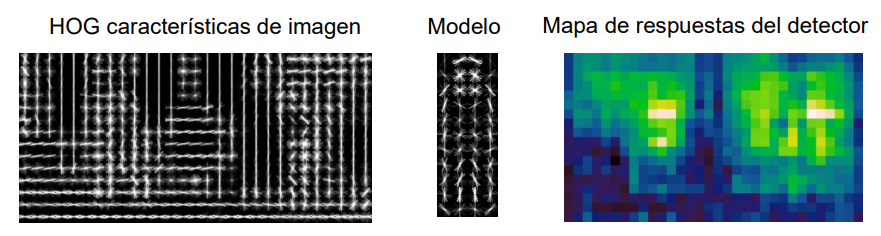
\includegraphics[width = \textwidth]{figs/deteccion-dalal.png}
\end{figure}

\begin{table}[h]
\centering
\begin{tabular}{p{6.5cm}|p{6.5cm}}
Ventajas del detector Dalal-Triggs & Desventajas del detector Dalal-Triggs \\ \hline
Funciona aceptablemente para objetos no deformables con orientaciones canónicas: caras, coches, personas & Requiere grandes cantidades de datos para entrenamiento \\
Detección rápida & No es robusto a oclusiones \\
 & Rendimiento bajo para objetos altamente deformables
\end{tabular}
\end{table}